% How to use writeLaTeX: 
%
% You edit the source code here on the left, and the preview on the
% right shows you the result within a few seconds.
%
% Bookmark this page and share the URL with your co-authors. They can
% edit at the same time!
%
% You can upload figures, bibliographies, custom classes and
% styles using the files menu.
%
%%%%%%%%%%%%%%%%%%%%%%%%%%%%%%%%%%%%%%%%%%%%%%%%%%%%%%%%%%%%%%%%%%%%%%

\documentclass[12pt,english,brazil]{article}
\usepackage{sbc-template}
\usepackage{adjustbox}
\usepackage{graphicx,url}
\usepackage{graphics}
\usepackage{color}
\usepackage{colortbl}
\usepackage[utf8]{inputenc}  
% Coloquei esse pacote para tamanho pequeno de fonte
\usepackage{scalefnt}
\usepackage{multirow}
\usepackage{subfigure}
\usepackage{multicol}
\usepackage{babel}
\babeltags{br = brazil, en = english}
\usepackage[T1]{fontenc}
\usepackage{xspace}
\usepackage{url}
\usepackage{enumerate}

\usepackage{xargs}
\usepackage[colorinlistoftodos,prependcaption,textsize=tiny]{todonotes}
\newcommandx{\ups}[2][1=]{\todo[linecolor=red,backgroundcolor=red!25,bordercolor=red,#1]{\tiny Gerson: #2}\xspace}
\newcommandx{\aham}[2][1=]{\todo[linecolor=yellow,backgroundcolor=yellow!25,bordercolor=yellow,#1]{\tiny Gui: #2}\xspace}
     
\sloppy

\title{Estudo de viabilidade do uso de Raspberry como servidor R-Shiny}

\author{Guilherme de Souza\inst{1}}


\address{Programa de Pós-Graduação em Computação \\Universidade Federal de Pelotas (UFPel)\\
  Caixa Postal 354 -- 96010.610 -- Pelotas -- RS -- Brazil
\nextinstitute
  Instituto de Matemática e Estatística (IME) -- Universidade de São Paulo (USP)\\
  Rua do Matão, 1010 -- São Paulo -- SP -- Brazil
  \email{\{gdsdsilva,gerson.cavalheiro\}@inf.ufpel.edu.br, gold@ime.usp.br}
}

\begin{document} 

\maketitle
    
\en
\begin{abstract}


\end{abstract}

\br
\begin{resumo} 


\end{resumo}



\section{Introdução}

Métricas de controle de qualidade e resultados ajudam a avaliar a confiança das previsões em estudos individuais.R é uma ferramenta livre que oferece grande potencial para manipulação e visualização de massas de dados. Shiny é um pacote para R que permite que servidores disponibilizem recursos para visualizações R. Existem outras, X e Y, que oferecem soluções semelhantes, porém, em um contexto proprietário.  Com arquitetura igualmente livre, a placa Raspberry Pi - um minicomputador que tem todo o seu hardware integrado em uma placa única, inicialmente desenvolvida em 2006 por Eben Upton e equipe (Werner 2015) - possui um custo baixo de aquisição, tamanho pequeno e baixo consumo energético. Ela é versátil, podendo ser usado para os mais diferentes tipos de aplicações, inclusive provendo serviços nativos a servidores (dados, web, serviços). Um dado interessante é que o Raspberry Pi 3 foi selecionado como o SBC (single board computer) mais popular, entre 81 placas Linux / Android, numa pesquisa abrangente conduzida pela Linux Foundation em 2016 (Brown, 2016.

Equipamentos servidores, independentemente das tarefas a que são submetidos, demandam consumo energético constante e ininterrupto e, por óbvio, é interessante buscar soluções que reduzam o uso de energia, provendo assim economia ou ganho financeiro.

Nesse interim, as métricas de desempenho, que são valores brutos que provem a base para alguma forma de pesquisa ou estudo e podem ser compostos por valores de diversas categorias e formato, tem a finalidade de quantificar objetivamente as funções de coletas de dados de avaliação e desempenho. Objetivamente, este trabalho busca avaliar e mensurar a o poder de escalabilidade de servidores web R, utilizando Shiny.

O caso de estudo encaminhado considera o serviço WebSYHDA. Um serviço desenvolvido com a finalidade de processamento complexo de séries hidrológicas. São consideradas duas plataformas de suporte: um servidor com arquitetura convencional e um dispositivo de baixa capacidade (small board). O objetivo deste estudo é identificar componentes do software, atualmente construído de forma monolítica, na forma de microserviços.

\section{Trabalhos Relacionados  - reescrito por Giovani rascunho para avaliação} \label{sec:TrabalhosRelacionados}

O estudo da escalabilidade de servidores no atendimento aos usuários é constante na literatura [citações
genéricas são bem vindas]. Nos últimos anos, esse estudo passou a incluir a análise das questões
energéticas [outras refs]. Neste contexto, o uso de dispositivos de borda, os chamados \emph{small
boards}, em substituição a servidores convencionais tem se apresentado como alternativa. No estudo de caso documento neste artigo, é considerada uma aplicação desenvolvida sob um servidor R.

Inicialmente, com um propósito similar ao WebSYHDA, no que tange ao uso de R e a estrutura Shiny, cita-se o  trabalho de Ekiz et al (2020) que utiliza os referidos recursos para criar uma aplicação web denominada Cluster Identity PRedictor (CIPR), disponível em GitHub, que fornece uma interface gráfica de usuário para pontuar perfis de expressão gênica de clusters de células.
Em outro contexto, a finalidade de criar um servidor de arquivos utilizando um Raspberry PI, para guardar os dados e poder compartilhar na rede, fora objeto de estudo de Bruschi (2016). Este concluiu que o dispositivo pode ser utilizado com o propósito em questão, com economia de custos sem, contudo, deixar de ser viável para esta aplicação, observando-se apenas algumas variações de desempenho dependendo do tipo de armazenamento.

O Raspberry Pi também foi utilizado, conforme Azevedo (2019), para propor a viabilidade de sua utilização em hospedar um honeypot, mostrando que sua efetividade irá depender da eficiência do software utilizado e também do tamanho e complexidade da rede em que ficará esse dispositivo, para dar efetividade ao objetivo proposto. Também dentro desse contexto de propor funcionalidades "servers" ao Raspberry Pi, Rafael et al (2013), outrora já mostrara que o uso de um computador de baixo custo - o Raspberry-Pi, pode ser usado de forma segura como um servidor web,  propiciando economia de energia.

[Oliveira and Ataides 2017] propôs avaliar a substituição do hardware convencional por um hardware de baixo consumo que respeite o Service-Level-Agreement (SLA) e reduza o consumo de energia dos data centers, assim tornando viável o uso de uma em uma nuvem computacional. A proposta incluiu a implementação de um Raspbarry PI B+ como um nodo computacional de baixo consumo energético. Para tal, adaptações na arquitetura e no hipervisor  se fizeram necessárias.

Para a elaboração deste compendio, os testes e medições foram realizados executando o bechmark YCSB Yahoo! Cloud Serving Benchmark, um sistema de código aberto e conjunto de programas para avaliar as capacidades de recuperação e manutenção de programas de computador. É frequentemente usado para comparar o desempenho relativo dos sistemas de gerenciamento de banco de dados NoSQL e nuvens. Com a análise das vazões das operações realizadas, pode-se perceber um gargalo de processamento quando comparado ao nó de um dispositivo de baixo consumo. Contudo, a implementação do Raspberry PI B+ em uma nuvem, ainda sim é vantajosa.

Em Kaup et al. (2014) é evidenciada segue a mesma preocupação com o alto consumo de energia proveniente de ambientes vindo das clouds. Ainda assim, até 2012, 10,82\% da população contribui com 0,03\% da energia consumida mundialmente, com o uso de 770 milhoes de gateways e routers domésticos. Levando em consideração que os maiores consumos ocorrem por parte de maquinas com um hardware mais poderoso, ainda sim não se pode ignorar o consumo vindo por parte de tais dispositivos, pois 43\% dos mesmos se mantem ligados diariamente, ociosos em boa parte do tempo, onde poderiam vir a desempenhar funções de pré-carregamento para usuário (ou seja, armazenamento em cache, pré-busca de conteúdo, execução de serviços locais). A Raspberry PI vem sendo utilizada para inúmeras aplicações no qual fomenta o uso de tais aplicações com a visão em baixo consumo energético. Kaup et al. (2014), apresenta o PowerPi um modelo de  potência concentrando-se no consumo de energia da Raspberry PI a fim de derivar novas possíveis estratégias de consumo de energia.



\section{WebSYHDA}\label{sec:websyhda}

%RASCUNHOOOOOOOOO
Engenharia e gestão de recursos hídricos mantém uma grande dependência de séries hidrológicas. No entanto, o processamento destas séries é complexo, geralmente dependente de métodos numéricos para resolução, e é suscetível a erros quando feito de forma manualmente. Esses aspectos frequentemente dificultam a elaboração de projetos que depende da análise e estudo de séries hidrológicas. Com isso O Grupo de Pesquisa em Hidrologia e Modelagem Hidrológica em Bacias Hidrográficas/CNPq da UFPEL, propôs, desenvolveu e mantem O \emph{System of Hydrological Data Acquisition and Analysis} ou SYHDA \cite{syhda}.

A plataforma recentemente passou por uma migração para o modelo Web, onde encontra-se em constante desenvolvimento. É integralmente desenvolvida em R, com auxílio do RStudio e de inúmeras bibliotecas gratuitas de uso geral, uso específico para a hidrologia e de funcionalidades para ambiente Web. %li no cobalto

O WebSYHDA permite a importação de dados do Hidroweb/ANA\footnote{ANA: \url{https://dadosabertos.ana.gov.br}}, para dados de vazão, chuva e nível. Estes dados são reconhecidos pela plataforma de forma automática. Outras fontes de dados estão sendo implementadas na plataforma, como BDMEP/INMET\footnote{INMET: \url{https://portal.inmet.gov.br}} e dados oriundos de estações de monitoramento diversas com formatos definidos pelo usuário.

% adicionei uma parte (joão)
A plataforma em sua versão atual, conta com diversas funcionalidades, bem como: constituição de séries históricas em diferentes intervalos de tempo, estatísticas descritivas, representações gráficas, testes não paramétricos, consistência de dados de chuva, análise de frequência local e análise de frequência regional. Os resultados serão estruturados de forma dinâmica, assim permitindo o manuseio pelo usuário final, permitindo ainda a possibilidade de exportação e salvar o estado atual do projeto. 

\subsection{Linguagem R} \label{sec:R}

R é uma linguagem e ambiente com foco em computação estatística e gráficos. Assim, R permite desenvolver e publicar gráficos bem projetados \cite{whatR}, semelhantemente a C/C++ e outras linguagens disponíveis no mercado, R também permite o desenvolvimento por meio de módulos, mas ainda se tratando de uma unica e grande aplicação.
%Colocar sobre a forma de escalabilidade do R aqui?!

Com isso vale ressaltar que R é uma aplicação de thread único, o que significa que um aplicativo não pode atender a dois usuários diferentes precisamente ao mesmo tempo, Figura ~\ref{singleThreads}. Em muitas aplicações isso não é um problema, porque a maioria dos cálculos leva apenas dezenas ou centenas de milissegundos. Como resultado, um único processo R geralmente pode atender de 5 a 30 solicitações por segundo \cite{ShinyappsEscalabilidade}. 

Entre tanto, para uma aplicação como o WebSYHDA e outras, onde a simultaneidade entre usuários podem ocorrer de forma frequente, acaba por resultar em respostas demoradas para os demais usuário, dado a dependência do tempo de processamento para o cálculo que estiver em execução. A fim de ganho em desempenho para compensar o número de usuários, o escalonamento de hardware pode ser feito, porem o emprego de \emph{hardware} para suporte pode ser empregada de forma pouco eficiente dado a configuração de balanceamento permitida. %De mesma maneira ocorre se houver o uso insuficiente, onde o custo por hardware ocioso deixa a desejar.

%Resaltar casos onde nao atenda

\begin{figure}[htbp]
  \centering 
  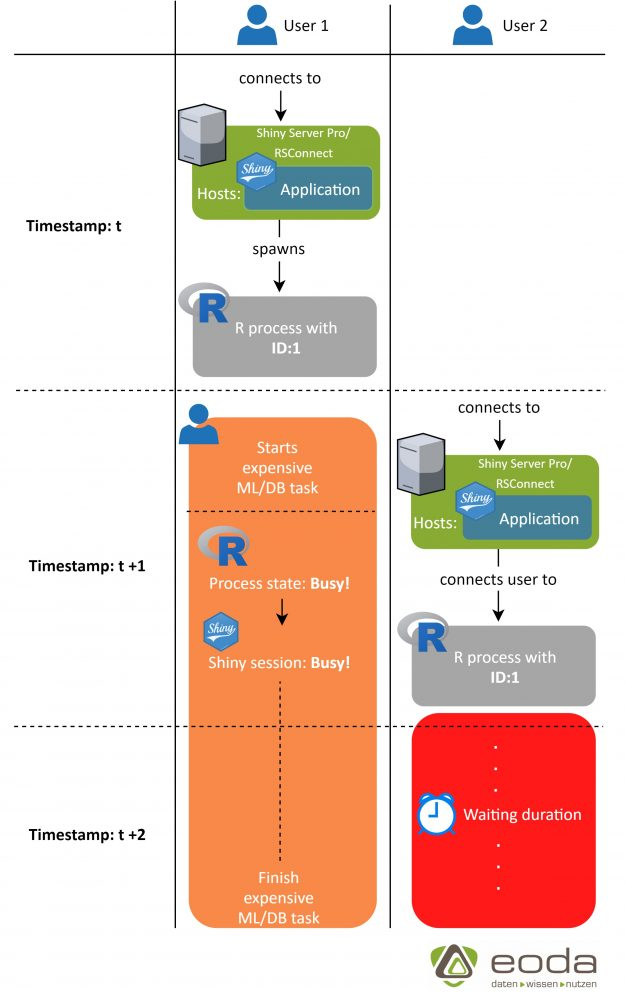
\includegraphics[scale=.4]{figures/single_threads.jpg}
  \caption{Exemplo de uma execução sequencial \cite{singleThreads}}
  \label{singleThreads}
\end{figure}

\subsection{Shiny} \label{sec:Shiny}

Para o desenvolvimento de aplicativos \emph{web} fazendo uso da linguagem R, a Rstudio mantém o pacote \emph{Shiny}\footnote{Shiny: \url{https://shiny.rstudio.com}}. Este pacote R que facilita a construção de aplicativos interativos. Permitindo hospedar aplicativos independentes em uma página da web ou incorporá-los em documentos R Markdown ou construir painéis. 

Assim, torna-se possivel apresentar gráficos dinâmicos e interativos por meio de pacotes como, ggvis\footnote{ggvis: \url{https://ggvis.rstudio.com/}}, ggiraph\footnote{ggiraph: \url{https://davidgohel.github.io/ggiraph}}, plotly\footnote{plotly: \url{https://plotly.com/}} entre outros mantidos pela RStudio ou pela comunidade. Permitindo ainda, estender os aplicativos \emph{Shiny} com temas CSS (\emph{Cascading Style Sheets}), \emph{htmlwidgets} e ações JS (\emph{JavaScript}).


\section{Metodologia} \label{sec:metodologia}

Visto que a demanda de serviços \textit{web} ocupa a maior parte das aplicações na nuvem, maiores são os esforços para otimização das aplicações para um menor consumo de requisitos e rede, mantendo, no entanto, níveis de desempenho aceitáveis aos usuários. 

Baseada na premissa supracitada, para este trabalho fizemos uso de uma aplicação real, o WebSYHDA como mecanismo de teste, que permitiu equiparar \emph{hardware} de arquitetura x64 com a \emph{smallboard} selecionado, Raspberry PI 3, dada a eficiência apresentada pelo dispositivo em trabalhos anteriores e a capacidade de atender cenários de demanda \emph{web} \cite{silva2019estudo}.

Para simulação de carga fizemos uso da ferramenta \emph{Shinycannon}, a qual nos permite simular usuários simultaneos realizando ações no aplicativo. Assim atendendo nossas exigências em quantativar numero de usuários suportados e latência do aplicativo.




\subsection{Shinycannon} \label{sec:Shinycannon}

\textit{Shinycannon}\footnote{Shinycannon: \url{https://github.com/rstudio/shinycannon}} é uma ferramenta de linha de comando que possibilita testes de carga em aplicativos R. Assim, permitindo aos desenvolvedores analisarem a escalabilidade de seu aplicativo simulando de um a n usuários simultaneos.

A ferramenta acompanha o pacote \textit{shinyloadtest}\footnote{Shinyloadtest: \url{https://rstudio.github.io/shinyloadtest}}, mantido pela própria Rstudio. O pacote é responsavel por gerar uma gravação de uma sessão de usuário, essas sessões podem ser criadas pensando no uso tipico do aplicativo desenvolvido\cite{shinyloadtest}. A sessão é criada de forma manual, após a inicialização do pacote o tester executa a interação com o aplicativo de forma natual, assim como um usuário comum. Ao terminar seu uso basta fechar a aplicação para que o pacote encerre a gravação da sessão.

Com isso, por sua vez, a \textit{Shinycannon} permite a criação de trabalhadores, que são os usuários simulados, podendo criar tantos quantos necessarios para execução dos testes. Assim para execução dos teste devemos definir o numero de trablhadores e o tempo total da sessão que será executada pelos mesmos. 

Em suma, a \textit{Shinycannon} replica os passos da gravação criada pelo pacote \textit{Shinyloadtest} entre seus trabalhadores (usuários), fazendo com que cada trabalhador execute simultaneamente a mesma sessão durante o tempo definido pelo desenvolvedor.

\subsection{Hardware}\label{sec:Hardware}
Com a popularização do uso de serviços providos pela computação em nuvem, o consumo energético dos data centers também aumentou, chegando a 270 TWh em 2012 \cite{VanHeddeghem:2014:TWI:2657027.2657141}, estimando chegar a mais de 2\% do consumo da energia mundial apos 2020 \cite{energy}.  Buscando alternativas de evitar esse alto consumo energético das máquinas convencionais utilizadas em data centers, o uso de dispositivos com arquitetura ARM, que possuem baixo consumo energético, são uma das estratégias possíveis.

Assim, o dispositivo de teste escolhido foi a \emph{smallboard} Raspberry PI3, dada sua arquitetura ARM aberta, comunidade participativa em inumeros projetos alem de sua alta disponbilidade no mercado. As especificacoes do device podem ser observadas na Tabela ~\ref{tab:especificacao}.

\begin{table}[h]
\centering
\caption{TESTE}
\begin{tabular}{l|c|c}
\hline
\multicolumn{1}{c|}{\textbf{Especifícação}}            & \textbf{Server x64} & \textbf{Raspberry PI3}                                                   \\ \hline
\textbf{Processador}                                   & XXX                 & \begin{tabular}[c]{@{}c@{}}BCM2837 64bit\\ Quad Core 1.2GHz\end{tabular} \\ \hline
\textbf{Arquitetura}   & XXX & ARMv8             \\ \hline
\textbf{RAM}           & XXX & 1 GB SDRAM 400MHz \\ \hline
\textbf{Armazenamento} & XXX & Micro SD          \\ \hline
\multicolumn{1}{c|}{\textbf{Máxima corrente / Tensão}} & XXX                 & 2.4A/5V                                                                  \\ \hline
\end{tabular}
\label{tab:especificacao}
\end{table}
    
Para comparativo de desempenho, utilizou-se um dispositivo de arquitetura x64.
O \textit{server} selecionado para tal comparativo, tem suas especificações presente na Tabela ~\ref{tab:especificacao}, informações obtidas pelo comando \textit{dmidecode}, o qual apresenta todas informações disponíveis sobre o dispositivo, possibilitando uma pesquisa mais especifica dentro dele atribuindo ao comando \textit{dmidecode --type} concatenado com uma chave da tabela de representação do comando, como a chave quatro, nos demonstrará todas especificações do processador e assim por diante.

\subsection{Metodologia dos Testes}\label{sec:MetodologiaDosTestes}
A fim de testar o aplicativo no seu estágio atual de desenvolvimento e também encontrar cargas próximas ao limite da Raspberry PI, consideramos a documentação como base, onde a mesma demonstra qual seria aproximadamente o limite de tempo de resposta do aplicativo dada a quantidade de usuários \cite{documentShiny}.


%Em um primeiro momento, analisamos o uso mais comum do sw, ou seja, seu uso diário por engenheiros hídricos, a Figura ~\ref{usoWebSYHDA} demonstra o conjunto de ações tomada dentro do aplicativo. Com isso utilizamos o pacote \emph{shinyloadtest}, assim permitindo a gravação deste conjunto de passos. 
Em um primeiro momento, buscou-se um teste que fosse característico de um fluxo típico de um usuário, fazendo uso de várias técnicas empregadas em diversas análises hidrológicas, porém com foco em tarefas que requerem maior processamento. Optou-se por utilizar o módulo de Análise de Frequência Regional para o teste, visto que o mesmo atende ao critério de uso anterior, assim como a exigência de múltiplos arquivos para computar os resultados. A Figura ~\ref{usoWebSYHDA} ilustra o conjunto de ações tomada para execução do teste dentro do aplicativo, sendo estas:

%A Figura ~\ref{usoWebSYHDA} ilustra o conjunto de ações tomada dentro do aplicativo. Com isso utilizamos o pacote \emph{shinyloadtest}, assim permitindo a gravação deste conjunto de passos. 

% descrição dos passos da Figura 2 (joão)
\begin{enumerate}[i.]
  \item Importar arquivos locais: importar 10 arquivos do Hidroweb, contendo dados de vazão;
  \item Aplicar filtros: aplicar o limiar de falhas de 31 dias para filtrar as séries;
  \item Constituir séries anuais: selecionar o período anual para transformar as séries diárias em anuais;
  \item Selecionar arquivos importados: no módulo de Análise de Frequência Regional, é possível selecionar, dentre os arquivos importados, quais serão utilizados na análise. Neste caso, todos foram selecionados;
  \item Análise de frequência regional: executar a análise. A partir dos dados, são computados os Momentos-L de cada série anual, as medidas de heterogeneidade da região e a sua função regional;
  \item Vizualizações geradas: tabelas com os resultados são geradas, assim como o gráfico da função regional.
\end{enumerate}



\begin{figure}[htbp]
  \centering 
  \includegraphics[scale=.4]{paperWSCAD2021/figures/useWebSYHDADrawio.png}
  \caption{Exemplo dos passos seguidos pelo usuário}
  \label{usoWebSYHDA}
\end{figure}

Inicialmente partimos com um conjunto de execuções teste afim de entender o simulador e as possibilidades fornecidas por ele. Seguindo as indicações da documentação e observando o tempo comum de trabalho de um usuário do \emph{WebSYHDA}, concluímos que %mudar isso
dois minutos representa mais de uma execução do conjunto de passos propostos, o que demonstra uma maior realidade de uso do aplicativo. Assim sendo, utilizamos dois minutos como limite de tempo de execução da ferramenta para nossa coleta.



%Nesses passos 10 arquivos foram utilizandos ... onde realiza ....

De forma semelhante, realizamos o aumento da carga parcialmente iniciando em um único trabalhador, logo após passamos a incrementar como demonstrado pela tabela ~\ref{tab:workers}. Para definição do limite de trabalhadores suportados, seguimos a documentação disponibilizada pela ferramenta, onde a mesma define que se aplicativos continuar sua execução muito tempo após a finalização do script, naturalmente ocasionam em respostas finais mais demoradas para o usuário final, assim, demonstrando a necessidade de recodificação do aplicativo ou o aumento de requisitos de \emph{hardware}. Todo o roteiro de testes e os arquivos gerados aqui apresentados, estão disponíveis no GitHub\footnote{GitHub: \url{https://github.com/SouzaGuilherme/research_PI3_R-Shiny-server}}.

\begin{table}[htbp]
\centering
\caption{Número de trabalhadores e tempo de simulação utilizados nos testes}
\begin{tabular}{c|c|cc}
\hline
\multicolumn{2}{c|}{\textbf{Servidor HP}} & \multicolumn{2}{c}{\textbf{Raspberry PI 3}}             \\ \hline
Trabalhadores     & Tempo                 & \multicolumn{1}{c|}{Trabalhadores} & Tempo              \\ \hline
1                 & \multirow{3}{*}{2}    & \multicolumn{1}{c|}{1}             & \multirow{3}{*}{2} \\ \cline{1-1} \cline{3-3}
10                &                       & \multicolumn{1}{c|}{4}            &                    \\ \cline{1-1} \cline{3-3}
20                &                       & \multicolumn{1}{c|}{}            &                    \\ \hline
\end{tabular}
\label{tab:workers}
\end{table}

\section{Resultados} \label{sec:Resultados}
Após a análise dos resultados obtidos a partir da execução do simulador nos cenários criados, focamos nos resultados de latência máxima de \emph{websocket}, ou seja, tempo de cálculo. Ressaltamos que os resultados aqui apresentados consideram os cenários e o estágio do aplicativo no momento de proposta deste trabalho. Para uma melhor visualização dos resultados, o próprio simulador desconsidera o tempo de aquecimento dos trabalhadores. Todos os resultados, estão disponíveis para consulta no GitHub\footnote{GitHub: \url{https://github.com/SouzaGuilherme/research_PI3_R-Shiny-server}} junto aos fontes.

Em um primeiro momento observamos a execucao com somente um trabalhador, Figura ~\ref{}, com o intuito de averiguar seu comportamento com somente um usuario ativo. Podemos obervar que a sessao mais lenta ficou em torno de 5s. Vale resaltar que o simulador reproduz os passos 

\section{Conclusão} \label{sec:conlusao}



\bibliographystyle{sbc}
\bibliography{sbc-template}

\end{document}
